\documentclass[a4paper,12pt]{article} % тип документа

% Поля страниц
\usepackage[left=2.5cm,right=2.5cm,
    top=2cm,bottom=2cm,bindingoffset=0cm]{geometry}
    
%Пакет дял таблиц   
\usepackage{multirow} 
    
%Отступ после заголовка    
\usepackage{indentfirst}


% Рисунки
\usepackage{floatrow,graphicx,calc}
\usepackage{wrapfig}

%%% Работа с картинками
\usepackage{graphicx}  % Для вставки рисунков
\graphicspath{{images/}{images2/}}  % папки с картинками
\setlength\fboxsep{3pt} % Отступ рамки \fbox{} от рисунка
\setlength\fboxrule{1pt} % Толщина линий рамки \fbox{}
\usepackage{wrapfig} % Обтекание рисунков и таблиц текстом

% Создаёем новый разделитель
\DeclareFloatSeparators{mysep}{\hspace{1cm}}

% Ссылки?
\usepackage{hyperref}
\usepackage[rgb]{xcolor}
\hypersetup{				% Гиперссылки
    colorlinks=true,       	% false: ссылки в рамках
	urlcolor=blue          % на URL
}


%  Русский язык
\usepackage[T2A]{fontenc}			% кодировка
\usepackage[utf8]{inputenc}			% кодировка исходного текста
\usepackage[english,russian]{babel}	% локализация и переносы




% Математика
\usepackage{amsmath,amsfonts,amssymb,amsthm,mathtools}

%%% Дополнительная работа с математикой
\usepackage{amsmath,amsfonts,amssymb,amsthm,mathtools} % AMS
\usepackage{icomma} % "Умная" запятая: $0,2$ --- число, $0, 2$ --- перечисление


% Что-то 
\usepackage{wasysym}


\begin{document}
\begin{center}
	\footnotesize{МОСКОВСКИЙ ФИЗИКО-ТЕХНИЧЕСКИЙ ИНСТИТУТ\\(НАЦИОНАЛЬНЫЙ 			ИССЛЕДОВАТЕЛЬСКИЙ УНИВЕРСИТЕТ)}\\
	\footnotesize{ФИЗТЕХ-ШКОЛА РАДИОТЕХНИКИ И КОМПЬЮТЕРНЫХ ТЕХНОЛОГИЙ\\}
	\hfill \break
	\hfill \break
	\hfill \break
	\hfill \break
	\hfill \break
	\hfill \break
\end{center}

\begin{center}   
    \hfill \break
	\hfill \break
	\hfill \break
	\hfill \break
	\hfill \break
	\hfill \break
	\hfill \break
	\hfill \break
	\hfill \break
	\hfill \break
	\hfill \break
	\large{Лабораторная работа № 3.5.1\\\large{\textbf{Изучение плазмы газового разряда в неоне}}}\\
	\hfill \break
	\hfill \break
	\hfill \break
	\hfill \break
	\hfill \break
	\hfill \break
	\hfill \break
	\hfill \break
	\hfill \break
	\hfill \break
	\hfill \break
	\begin{flushright}
		Климова Екатерина\\
		Группа Б01-108
	\end{flushright}
	\hfill \break
\end{center}
\hfill \break
\hfill \break
\begin{center}
	Долгопрудный, 2022 г.
\end{center}
\thispagestyle{empty}

\newpage
\hfill \break
\textbf{Цель работы:} изучение вольт-амперной характеристики тлеющего разряда; изучение свойств плазмы методом зондовых характеристик.
\hfill \break
\hfill \break
\textbf{В работе используются:} стеклянная газоразрядная трубка, наполненная неоном;  высоковольтный источник питания; источник питания постоянного тока; делитель напряжения; потенциометр; амперметры; вольтметры; переключатели.

\section{Аннотация}
\hfill \break В работе предлагается измерить вольт-амперную характеристику тлеющего разряда и зондовые характеристики при разных токах разряда. По результатам измерений рассчитать концентрацию и температуру электронов в плазме, степень ионизации, плазменную частоту и дебаевский радиус экранирования.

\section{Теоретическое введение}
\hfill \break Как известно, вещество может находиться в трех агрегатных состояниях $-$ твердом, жидком или газообразном, причем эти состояния последовательно сменяются при возрастании температуры. Если и дальше нагревать газ, то сначала молекулы диссоциируют на атомы, а затем и атомы распадаются на электроны и ионы, так что газ становится \textit{ионизованным}, представляя собой смесь из свободных электронов и ионов, а также нейтральных частиц. Если степень ионизации газа (отношение числа ионизованных частиц к общему их числу) оказывается достаточно велика, то поведение заряженных частиц принимает коллективный характер, так что описание свойств среды не может быть сведено к описанию обычного газа. Такое состояние ионизованного газа называется \textbf{плазмой}.

\hfill \break Из характерных свойств плазмы можно выделить высокую электропроводность и квазинейтральность. Частицы в плазме стараются распределиться таким образом, чтобы средняя плотность заряда была равна нулю. Равенство концентраций положительных и отрицательных частиц $-$ квазинейтральность $-$ нарушается, как правило, лишь в микроскопических масштабах из-за тепловых флуктуаций. 

\hfill \break В низкотемпературной плазме ($T \approx 10^4$ К) степень ионизации атомов обычно невелика. Например, в тлеющем газовом разряде (при низком давлении газа и малом токе) люминисцентной лампы концентрация электронов составляет $n_{e} \approx 10^9 \text{ см}^{-3}$, а концентрация нейтральных молекул $-$ $n_{0} \approx 10^{14} \text{ см}^{-3}$. Лишь внутри звезд и в некоторых установках, где температуры достигают $T \approx 10^6$ К и более, доля ионизованных атомов приближается к единице. 

\hfill \break Стационарное состояние плазмы часто является неравновесным. При этом электроны и ионы в плазме, как правило, имеют разную температуру. Это связано с тем, что масса электрона много меньше массы иона, поэтому при электрон-ионных столкновениях обмен энергией идет гораздо медленне, чем при столкновениях частиц одного сорта. Например, в тлеющем газовом разряде обычно имеются <<холодные>> ионы и <<горячие>> электроны. Так получается из-за того, что в сильно разреженном газе электроны ускоряются внешним электрическим полем, почти не теряя энергии при соударениях с ионами и атомами газа или стенками сосуда, $-$ в результате электроны разгоняются до высоких температур $T_{e} \approx 10^4$ К. Ионы же, напротив, быстро отдают полученную от поля и от электронов энергию нейтральным атомам газа и атомам стенок, поскольку их массы близки, $-$ поэтому их температура оказывается порядка комнатной ($T_{i} \approx 300$ К).

\subsection{Плазменная частота}

\begin{wrapfigure}{l}{0.3\textwidth}
\begin{center}
    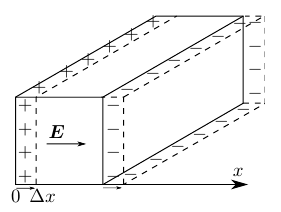
\includegraphics[width=1\textwidth]{3.5.1_1.png}
    \textbf{Рис. 1.} Плазменные колебания
\end{center}
\end{wrapfigure}

\hfill \break Выделим в нейтральной плазме некоторый объем в виде параллелепипеда (рис. 1); обозначим концентрацию электронов как $n_{e}$; ионы для простоты будем считать однозарядными (в уравнении квазинейтральности плазмы $-en_{e}+(Ze)n_{i} = 0$ количество электронов, которое отдает в плазму каждый ион, $Z = 1$), тогда $n_{e} = n_{i}$. Предположим, что все электроны сместились на расстояние $x$ относительно ионов. Ионы же весят существенно больше, поэтому их можно считать неподвижными. В результате на боковых гранях пераллелепипеда возникнут нескомпенсированные поверхностные заряды с плотностью $\pm n_{e}e\Delta x$, которые, как две пластины конденсатора, создадут электрическое поле, которое будет действовать на электроны, придавая им ускорение:

$$
\Delta \ddot{x} = -\frac{eE}{m_{e}} = -\frac{4\pi n_{e}e^2}{m_{e}} \Delta x.
$$

\hfill \break Видно, что полученное уравнение описывает гармонические колебания с частотой

\begin{equation}\label{ linkname }
\omega_{p} = \sqrt{\frac{4\pi n_{e}e^2}{m_{e}}}.
\end{equation}

\hfill \break Таким образом, мы получили частоту коллективных колебаний электронов относительно квазинейтрального состояния. Такие колебания называют ленгмюровскими, а частоту $\omega_{p}$ $-$ плазменной или \textit{ленгмюровской}. Эта частота $-$ один из важнейших параметров плазмы, потому что она определяет характерный временной масштаб для плазмы $-$ время отклика на флуктуацию плотности заряда в ней.

\subsection{Дебаевский радиус}

\hfill \break Оценим амплитуду плазменных колебаний, возбужденных за счет тепловой энергии, содержащейся непосредственно в плазме. 

\hfill \break Средняя скорость теплового движения электронов по порядку величины равна $\bar v_{e} \approx \sqrt{k_\text{Б}T_{e}/m_{e}}$. Тогда искомая амплитуда

\begin{equation}\label{ linkname }
r_{D} = \sqrt{\frac{k_\text{Б}T_{e}}{4\pi n_{e}e^2}} \approx \frac{\bar v_{e}}{\omega_{p}}
\end{equation}

\hfill \break называется \textit{дебаевским радиусом} и характеризует пространственный масштаб многих плазменных явлений. Также видно, что дебаевский радиус есть амплитуда ленгмюровских колебаний, возбуждаемых тепловыми флуктуациями. Он задает масштаб, на котором возможно спонтанное нарушение квазинейтральности плазмы.

\subsection{Плазменное экранирование}

\hfill \break Поместим в равновесную плазму с температурой $T = T_{e} = T_{i}$ некоторую пробную частицу, имеющую фиксированный положительный заряд $+q$, и найдем, как распределятся заряженные плазменные частицы вокруг нее. Будем считать, что частица достаточно массивна, так что ее можно считать неподвижной.

\begin{wrapfigure}{r}{0.3\textwidth}
\begin{center}
    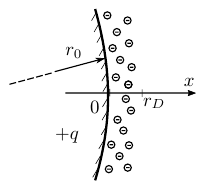
\includegraphics[width=1\textwidth]{3.5.1_2.png}
    \textbf{Рис. 2.} Упрощенная геометрия задачи об экранировании заряда
\end{center}
\end{wrapfigure}

\hfill \break Заряд будет притягивать к себе плазменные электроны, в результате чего вокруг него образуется <<облако>>, заряженное отрицательно и \textit{экранирующее} поле заряда на большом расстоянии от него $-$ электрическое поле вокруг $q$ будет быстрее убывать, чем по закону $q/r^2$. Если бы электроны не имели кинетической энергии, то они так <<облепили>> бы пробный заряд, что его собственное поле было бы полностью скомпенсировано. Тепловое движение мешает такой компенсации.

\hfill \break Чтобы наглядно выявить характерные особенности данной задачи, предположим, что радиус $r_{0}$ пробной частицы велик по сравнению с дебаевским и будем рассматривать распределение поля вдоль ее поверхности $-$ так мы сведем задачу к одномерной.

\hfill \break Пространственное распределение электронов в равновесии подчиняется распределению Больцмана:

$$
n_{e} = n_{e0} \cdot \exp{\frac{e\varphi}{k_\text{Б}T}},
$$

\hfill \break где $\varphi$ $-$ потенциал электростатического поля, $n_{e0}$ $-$ концентрация электронов вдали от заряда, где $\varphi \rightarrow 0$. Будем считать, что температура электронов в плазме настолько велика, что 

$$
\frac{e\varphi}{k_\text{Б}T} \ll 1.
$$

\hfill \break Найдем объемную плотность заряда:

$$
\rho = -en_{e}+en_{i} \approx -en \cdot \frac{e\varphi}{k_\text{Б}T},
$$

\hfill \break где $n = n_{e0} + n_{i0} = 2n_{e0}$ $-$ полная концентрация заряженных частиц вдали от $q$. Запишем уравнение Пуассона для одномерного случая:

$$
\frac{d^2\varphi}{dt^2} = -4\pi \rho.
$$

\hfill \break Учитывая граничные условия ($\varphi(\infty) = 0$ и $\varphi(0) = \frac{q}{r_0}$), получим

\begin{equation}\label{ linkname }
\varphi(x) = \frac{q}{r_{0}}e^{-\frac{x}{r_{D}}}.
\end{equation}

\hfill \break Таким образом, потенциал поля и его напряженность, а также концентрация плазменных частиц изменяются при удалении от пробного заряда по экспоненциальному закону с характерной длиной порядка дебаевского радиуса. На расстояниях, превышающих эту длину, плазму фактически можно считать квазинейтральной, а поле заряда $q$ практически экранированным. В связи с этим дебаевский радиус также называют \textit{радиусом экранирования}.

\begin{center}
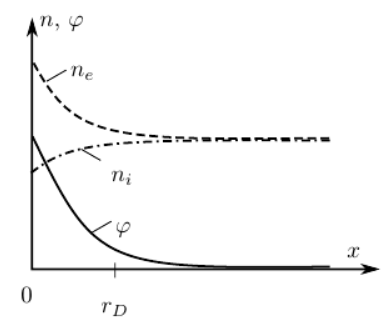
\includegraphics[width=0.45\linewidth]{3.5.1_3.png}\\
\textbf{Рис. 3.} Схематичное распределение потенциала (сплошная) и плазменных зарядов (пунктиры)\\
\end{center}

\hfill \break Теперь можно дать количественное определение плазмы. \textbf{Плазмой} называется ионизованный газ, дебаевский радиус которого существенно меньше характерного размера области $a$, занимаемой этим газом:

$$
\sqrt{\frac{k_\text{Б}T}{4\pi ne^2}} \ll a.
$$

\hfill \break Именно при таком соотношении поведение среды носит коллективный характер. \textit{Идеальной} называется плазма, энергия кулоновского взаимодействия частиц которой мала по сравнению с тепловой. Это выполняется, если в дебаевской сфере число частиц велико. Идеальную плазму можно с хорошей точностью рассматривать как идеальный газ.

\subsection{Плавающий потенциал}

\hfill \break Для исследования свойств плазмы используется зондовый метод. Зонд, представляющий собой небольшой проводник, помещается в плазму и измеряет электрический потенциал. Измерив вольт-амперную характеристику зонда, можно определить температуру плазмы, её дебаевский радиус и ленгмюровскую частоту.
    
\hfill \break При внесении проводника в плазму он подвергается бомбардировке заряженными частицами, преимущественно электронами. Будем считать плазму идеальной. Тогда поток электронов на единичную поверхность (число частиц, ударяющихся о единичную поверхность за одну секунду) равен:

$$
j = \frac{1}{4} n \bar v,
$$

\hfill \break где $\bar v = \sqrt{\frac{8 k T}{\pi m}}$ $-$ средняя тепловая скорость движения частиц. Так как скорость электронов больше скорости ионов, то проводник зарядится отрицательно и приобретет отрицательный потенциал $-U_f$, называемый \textit{плавающим потенциалом}.
    
\hfill \break В начальный момент времени потенциал зонда равен $0$, тогда электронный и ионный токи, которые называют \textit{тепловыми} равны:

$$
I_{e0} = -\frac{n \bar v_e}{4} eS, \hspace{2mm} I_{i0} = \frac{n \bar v_i}{4} eS,
$$
    
\hfill \break где $S$ $-$ площадь зонда, $n = n_{e} = n_{i}$. Когда потенциал зонда станет равен $-U_f$, то электроны будут замедляться зондовым полем, ионы ускорятся. Так как масса ионов большая, то потенциальный барьер зонда практически не повлияет на ионный ток:
    
$$
I_i \approx I_{i0}.
$$
    
\hfill \break Электронный ток уменьшится, так как только электроны, обладающие достаточной кинетической энергией, способны преодолеть потенциальный барьер. Так как распределение электронов по энергии определяется распределением Больцмана, то электронный ток равен
    
$$
I_{e} = I_{e0} \exp \left( -\frac{e U_f}{kT_e} \right).
$$
    
\hfill \break В состоянии равновесия электронный и ионный токи равны $I_e = I_i$. Тогда

\begin{equation}\label{ linkname }
U_f = -\frac{kT}{e} \ln{\frac{\bar v_i}{\bar v_e}} = \frac{1}{2} \frac{kT}{e} \ln{\frac{T_e m_i}{T_i m_e}}.
\end{equation}

\begin{center}
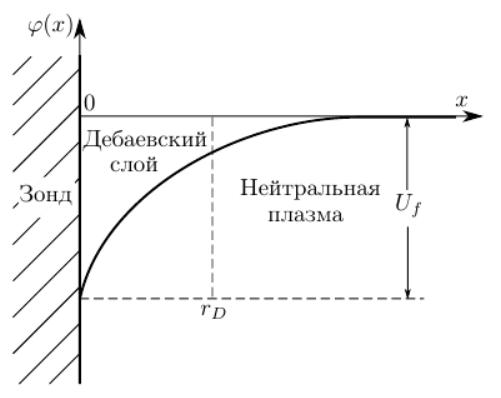
\includegraphics[width=0.45\linewidth]{3.5.1_4.png}\\
\textbf{Рис. 4.} Распределение потенциала в окрестности зонда\\
\end{center}
    
\subsection{Измерение с помощью двойного зонда}
    
\hfill \break \textit{Двойным зондом} называется система, состоящая из двух зондов, расположенных на небольшом расстоянии друг от друга. Между зондами создаётся разность потенциалов $U$, которая по величине много меньше плавающего потенциала. При этом оба зонда имеют близкий к плавающему потенциал.

\hfill \break При отсутствии разности потенциалов ток между зондами равен нулю. Рассчитаем величину тока, проходящего через двойной зонд вблизи точки $I = 0$. При небольших разностях потенциалов ионные токи на оба зонда равны ионному току насыщения (формула Бома: $I_{i\text{н}} \approx 0.4n_{i}eS\sqrt{\frac{2k_\text{Б}T_{e}}{m_{i}}}$) и компенсируют друг друга. Величина результирующего тока целиком связана с различием в электронных токах. Пусть
    
\begin{equation}\label{ linkname }
    \begin{split}
    	U_1 &= U_f + \Delta U_1 \\
    	U_2 &= U_f + \Delta U_2,
    \end{split}
\end{equation}

\hfill \break где $U_1$ $-$ потенциал первого зонда, $U_2$ $-$ потенциал второго зонда, $\Delta U_1, \Delta U_2 \ll U_f$. Напряжение $U$ между зондами равно
    
$$
U = \Delta U_2 - \Delta U_1.
$$
    
\hfill \break Вольт-амперная характеристика зонда представлена на рис. (5). Приближенная зависимость, описывающая вольт-амперную характеристику двойного зонда:
    
\begin{equation}
I = I_{i\text{н}} \th \left( \frac{eU}{2 kT_e} \right).
\end{equation}

\hfill \break \textit{Током насыщения} называется ток, которому соответствует точка пересечения наклонной асимптоты и оси ординат. На левой ветви в пределе $U \rightarrow - \infty$ электронный ток прекращается $I_e \rightarrow 0$, на правой ветви  $U \rightarrow \infty$ прекращается ионный ток из-за потенциального барьера. Электронный ток насыщения можно оценить по формуле
    
$$
I_{e\text{н}} \approx I_{e0} \approx \frac{1}{4} n_e S \sqrt{\frac{8 kT}{\pi m_e}}.
$$
    
\hfill \break Из графика (5) сначала находится ионный ток насыщения $I_{i\text{н}}$ из пересечения асимптот с осью $U = 0$. Затем находится наклон графика в начале координат, из которого можно определить температуру электронов $T_{e}$. Дифференцируя (5) по $U$ в точке $U = 0$ и принимая во внимание, что при малых аргументах $\th x \approx x$, найдем

\begin{equation}\label{ linkname }
k_\text{Б}T_{e} = \frac{1}{2} \frac{eI_{i\text{н}}}{\frac{dI}{dU}|_{U=0}},
\end{equation}

\hfill \break где $\frac{dI}{dU}$ $-$ наклон характеристики зонда вблизи начала координат. По известным $T_{e}$ и $I_{i\text{н}}$ можно найти концентрацию заряженных частиц $n_{i} = n_{e}$ по формуле Бома.

\hfill \break Таким образом, двойные зонды удобно применять для измерения электронной температуры и концентрации частиц в плазме.
    
\begin{center}
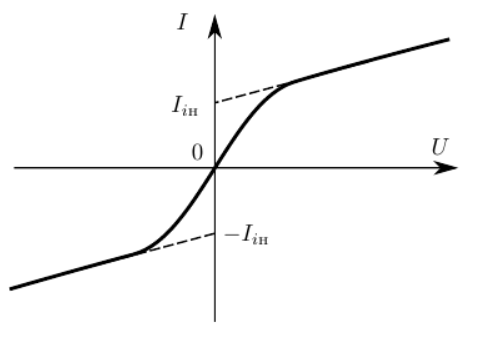
\includegraphics[width=0.50\linewidth]{3.5.1_5.png}\\
\textbf{Рис. 5.} Вольт-амперная характеристика двойного зонда\\
\end{center}

\section{Экспериментальная установка}
\hfill \break Схема установки для исследования плазмы газового разряда в неоне изображена на рис. 6. Стеклянная газоразрядная трубка имеет холодный (ненагреваемый) полый катод, три анода и геттерный узел $-$ стеклянный баллон, на внутреннюю поверхность которого напылена газопоглощающая пленка (геттер). Трубка наполнена изотопом неона $^{22}Ne$ при давлении $2$ мм рт. ст. Катод и один из анодов (I или II) с помощью переключателя $\text{П}_{1}$ подключаются через балластный резистор $R_\text{б} \approx 450$ кОм к регулируемому высоковольтному источнику питания (ВИП) с выходным напряжением до $5$ кВ.

\begin{center}
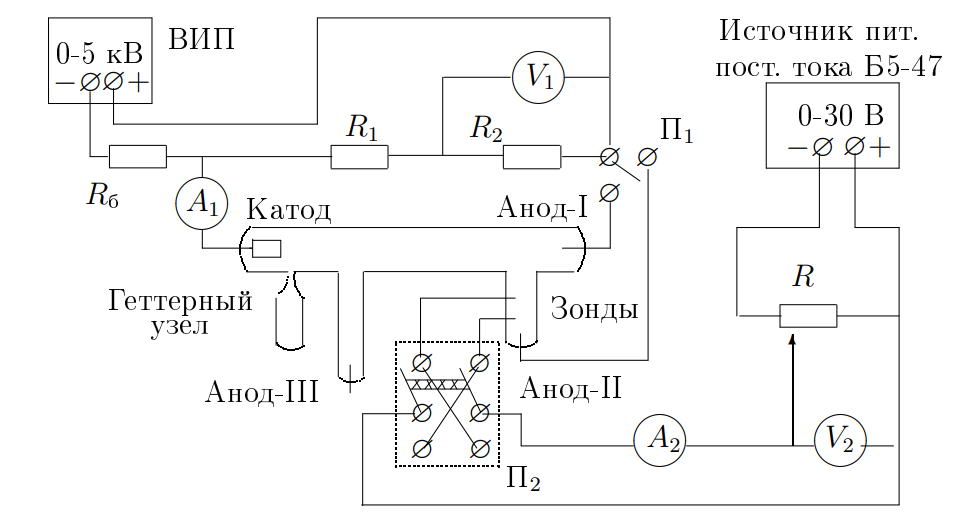
\includegraphics[width=0.75\linewidth]{3.5.1_6.png}\\
\textbf{Рис. 6.} Схема установки для исследования газового разряда\\
\end{center}

\hfill \break При подключении к ВИП анода-I между ним и катодом возникает газовый разряд. Ток разряда измеряется миллиамперметром $A_{1}$, а падение напряжения на разрядной трубке $-$ цифровым вольтметром $V_{1}$ (мультиметром $GDM$), подключенным к трубке через высокоомный ($2$5 МОм) делитель напряжения с коэффициентом $(R_{1}+R_{2})/R_{2} = 10$.

\hfill \break При подключении к ВИП анода-II разряд возникает в пространстве между катодом и анодом-II, где находится двойной зонд, используемый для диагностики плазмы положительного столба.

\hfill \break Зонды изготовлены из молибденовой проволоки диаметром $d = 0.2$ мм и имеют длину $l = 5.2$ мм. Они подключены к источнику питания $GPS$ через потенциометр $R$. Переключатель $\text{П}_{2}$ позволяет изменять полярность напряжения на зондах. Величина напряжения на зондах измеряется с помощью дискретного переключателя $V$ выходного напряжения источника питания и потенциометра $R$, а измеряется цифровым вольтметром $V_{2}$ ($GDM$). Для измерения зондового тока используется мультиметр $A_{2}$ ($GDM$). Анод-III в нашей работе не используется.

\section{Ход работы}

\subsection{Вольт-амперная характеристика разряда}
\hfill \break Подготовим приборы к работе в соответствии с техническим описанием. Плавно увеличивая выходное напряжение ВИП, определим напряжение зажигания заряда, то есть напряжение, которое показывал вольтметр $V_{1}$ непосредственно перед зажиганием: $U_\text{заж} = 220$ В. 

\hfill \break С помощью вольтметра $V_{1}$ и амперметра $A_{1}$ снимем вольт-амперную характеристику разряда $I_{p}(U_{p})$, результаты занесем в таблицу 1:

\begin{center}
\begin{tabular}{|c|c|}\hline
$ U_{p} $, В & $ I_{p} $, мА \\\hline
36.25 & 0.19 \\\hline
35.14 & 0.39 \\\hline
33.87 & 0.58 \\\hline
33.03 & 0.77 \\\hline
32.49 & 0.97 \\\hline
32.06 & 1.16 \\\hline
31.76 & 1.35 \\\hline
31.06 & 1.55 \\\hline
30.04 & 1.74 \\\hline
29.63 & 1.94 \\\hline
29.03 & 2.13 \\\hline
28.53 & 2.32 \\\hline
28.04 & 2.52 \\\hline
27.69 & 2.71 \\\hline
27.53 & 2.90 \\\hline
27.39 & 3.10 \\\hline
27.23 & 3.29 \\\hline
27.11 & 3.48 \\\hline
27.08 & 3.68 \\\hline
27.06 & 3.87 \\\hline
27.06 & 4.06 \\\hline
27.11 & 4.26 \\\hline
27.12 & 4.45 \\\hline
27.06 & 4.65 \\\hline
27.04 & 4.84 \\\hline
\end{tabular} \\
\hfill \break \textbf {Таблица 1.} Вольт-амперная характеристика разряда\\
\end{center}

\hfill \break Построим ВАХ разряда в координатах $U_{p}(I_{p})$:

\begin{center}
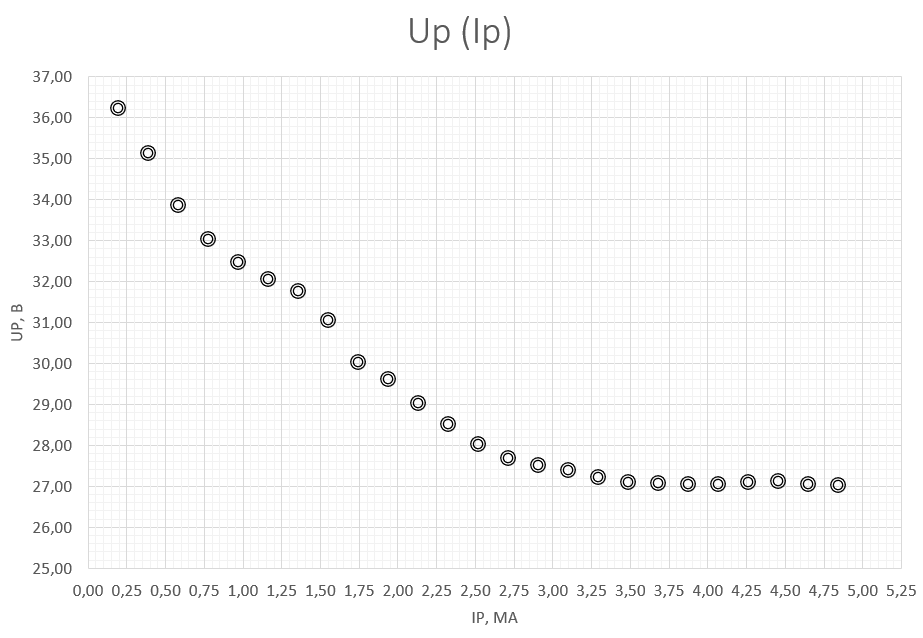
\includegraphics[width=0.85\textwidth]{3.5.1_7.png}\\
\textbf{Рис. 7.} График вольт-амперной характеристики разряда \\
\end{center}

\hfill \break Зная максимальный наклон графика, можно найти максимальное дифференциальное сопротивление разряда $R_\text{диф} = dU/dI$. Максимальный наклон график будет иметь в первых трех своих точках:

\begin{center}
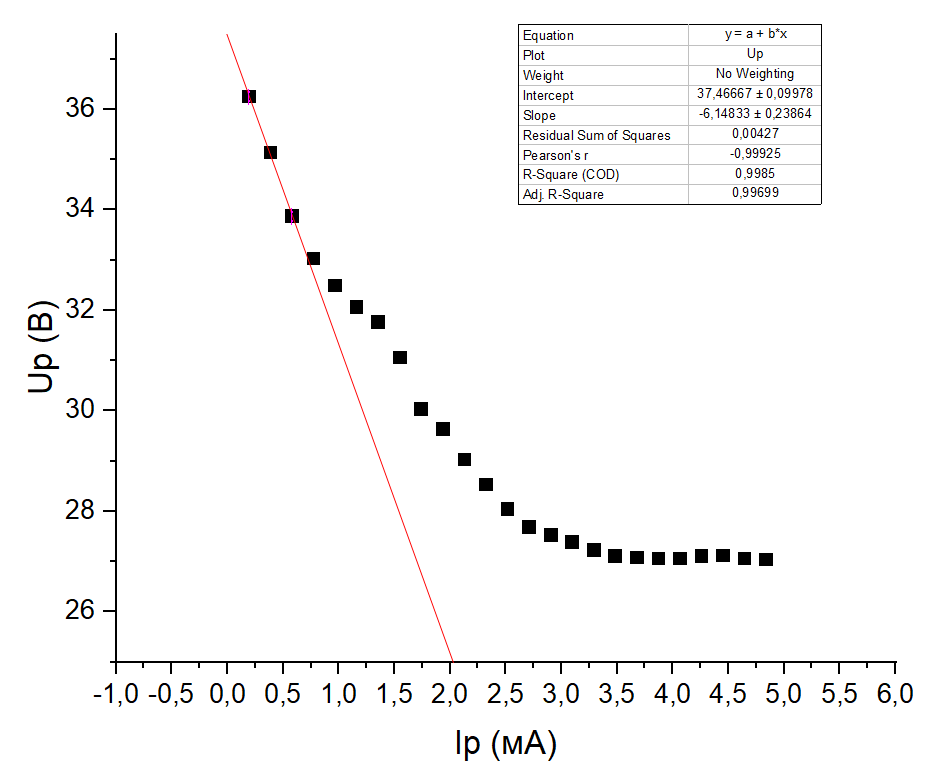
\includegraphics[width=0.95\textwidth]{3.5.1_8.png}\\
\textbf{Рис. 8.} График вольт-амперной характеристики разряда; максимальный наклон \\
\end{center}

\hfill \break Отсюда видно, что (учитывая, что вольтметр подключен через делитель напряжения с коэффициентом 10) $|R_\text{диф}| = (6.15 \pm 0.24) \cdot 10^4$ Ом. Конечно, в определении погрешности значения сопротивления должна также сыграть роль погрешность определения тока на амперметре и напряжения на вольтметре, но они малы по сравнению с указанной выше.

\subsection{Зондовые характеристики}

\hfill \break Уменьшим напряжение ВИП до нуля, а затем будем плавно увеличивать до возникновения разряда. Установим максимальное значение разрядного тока $I_{p} = 5$ мА и максимальное напряжение на зонде $U_\text{з} = 25$ В. Измерим c помощью вольтметра $V_{2}$ и амперметра $A_{2}$ вольт-амперную характеристику двойного зонда $I_\text{з} (U_\text{з})$ при трех различных фиксированных токах разряда $I_{p}$ $-$ 5 мА, 3 мА и 1.5 мА на амперметре $A_{1}$. Измерения будем проводить в диапазоне от $-U_{max} = -25$ В до $+U_{max} = 25$ В, меняя полярность подключения зонда при нулевом токе. Занесем полученные зондовые характеристики в таблицу 2:

\begin{center}
\begin{tabular}{|c|c|c|c|c|c|}\hline
$U_\text{з}$, В & $I_\text{з}$, мкА & $U_\text{з}$, В & $I_\text{з}$, мкА & $U_\text{з}$, В & $I_\text{з}$, мкА \\\hline
\multicolumn{2}{|c}{$I_p$ = 5.0 мА} & \multicolumn{2}{|c}{$I_p$ = 3.0 мА} & \multicolumn{2}{|c|}{$I_p$ = 1.5 мА} \\\hline
 25.04 &   92.78 &  25.03 &  54.32 &  25.02 &  30.02 \\\hline
 22.00 &   87.98 &  22.01 &  54.32 &  21.99 &  28.75 \\\hline
 18.99 &   85.18 &  19.00 &  52.27 &  19.02 &  27.50 \\\hline
 16.01 &   81.73 &  16.00 &  50.04 &  15.99 &  26.23 \\\hline
 13.00 &   76.44 &  13.01 &  47.59 &  13.00 &  24.88 \\\hline
  9.97 &   68.21 &  10.00 &  43.71 &  10.01 &  22.97 \\\hline
  8.00 &   60.09 &   7.99 &  39.41 &   8.01 &  20.87 \\\hline
  5.95 &   49.05 &   6.01 &  33.10 &   6.02 &  17.77 \\\hline
  3.95 &   34.86 &   4.00 &  24.32 &   4.00 &  13.34 \\\hline
  2.03 &   19.78 &   2.01 &  13.28 &   2.00 &   7.49 \\\hline
  0.94 &    9.96 &   0.98 &   6.59 &   0.99 &   4.09 \\\hline
  0.01 &    0.73 &   0.00 &   0.00 &   0.01 &   0.57 \\\hline
 -0.01 &    0.88 &  -0.01 &  -0.61 &  -0.01 &   0.00 \\\hline
 -0.96 &   -8.37 &  -1.01 &  -7.66 &  -1.00 &  -3.61 \\\hline
 -1.99 &  -18.78 &  -2.00 & -14.42 &  -1.99 &  -7.15 \\\hline
 -4.00 &  -38.00 &  -4.01 & -27.02 &  -4.01 & -13.70 \\\hline
 -6.00 &  -54.70 &  -5.98 & -37.16 &  -6.03 & -19.03 \\\hline
 -8.00 &  -68.06 &  -8.00 & -44.99 &  -8.01 & -22.86 \\\hline
 -9.99 &  -78.09 & -10.00 & -50.43 & -10.02 & -25.48 \\\hline
-13.00 &  -87.98 & -13.00 & -55.04 & -13.00 & -27.58 \\\hline
-16.03 &  -93.86 & -16.00 & -57.33 & -16.00 & -28.56 \\\hline
-18.98 &  -97.30 & -18.99 & -59.25 & -19.00 & -29.35 \\\hline
-22.01 & -100.60 & -22.03 & -60.86 & -21.99 & -30.14 \\\hline
-25.04 & -103.96 & -25.03 & -62.78 & -25.03 & -30.99 \\\hline
\end{tabular} \\
\hfill \break \textbf {Таблица 2.} Зондовые характеристики при различных значениях тока разряда\\
\end{center}

\hfill \break Построим зондовые характеристики $I_\text{з} = f(U_\text{з})$, отцентрируем кривые и с их помощью найдем температуры электронов $T_{e}$ по формуле (7):

$$
T_{e} = \frac{1}{2k} \frac{eI_{i\text{н}}}{\frac{dI}{dU}|_{U=0}},
$$

\hfill \break где ток $I_{i\text{н}}$ можно найти из перечения асимптоты к току насыщения с осью $U = 0$ (рис. 9), $\frac{dI}{dU}_{U=0}$ $-$ наклон $I = f(U)$ в начале координат, $kT_{e} = (\Delta U)/2$ эВ, $\Delta U$ $-$ расстояние между абсциссами точек пересечения асимптот на графиках на рис. 9. 

\begin{center}
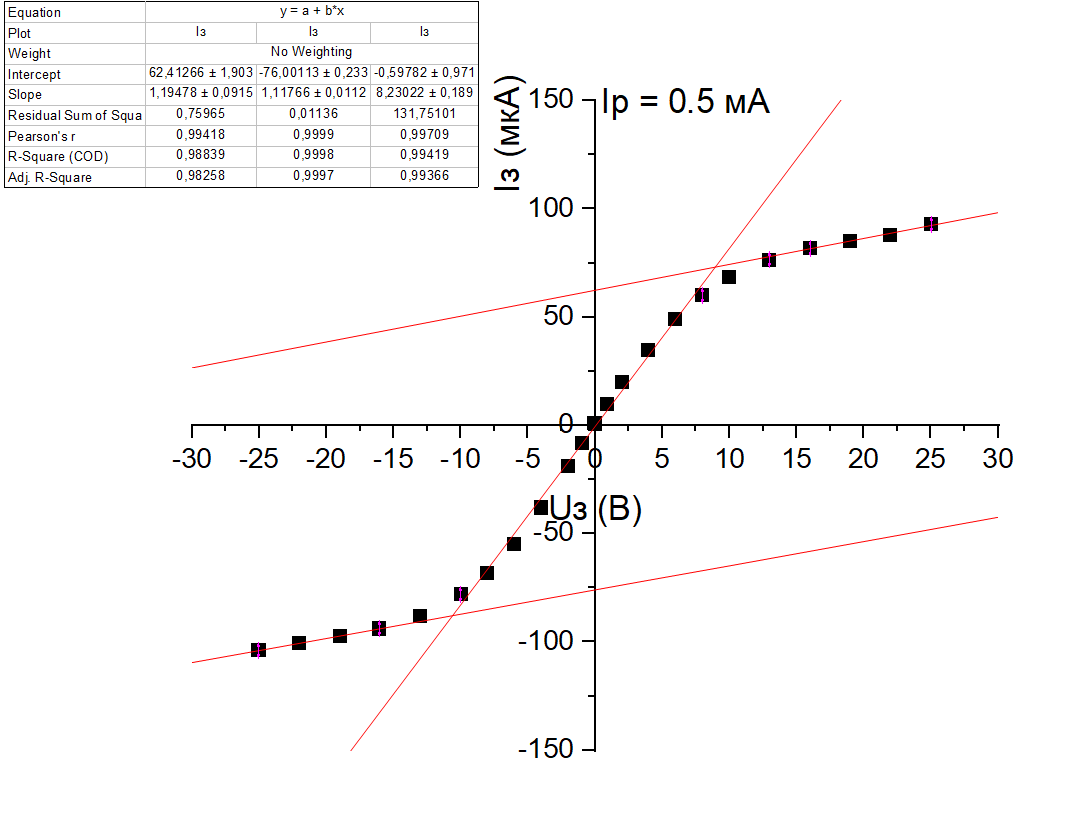
\includegraphics[width=0.95\textwidth]{3.5.1_9.png}\\
(а) ВАХ двойного зонда, $I_{p} = 5.0$ мА  \\
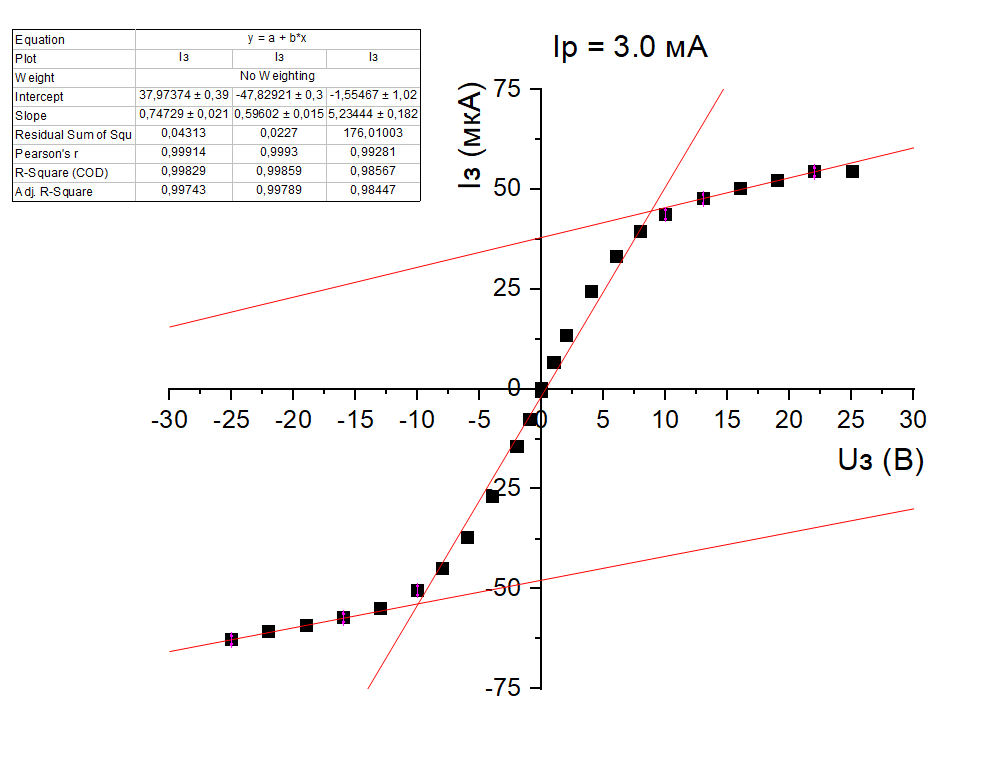
\includegraphics[width=0.95\textwidth]{3.5.1_10.png}\\
(b) ВАХ двойного зонда, $I_{p} = 3.0$ мА  \\
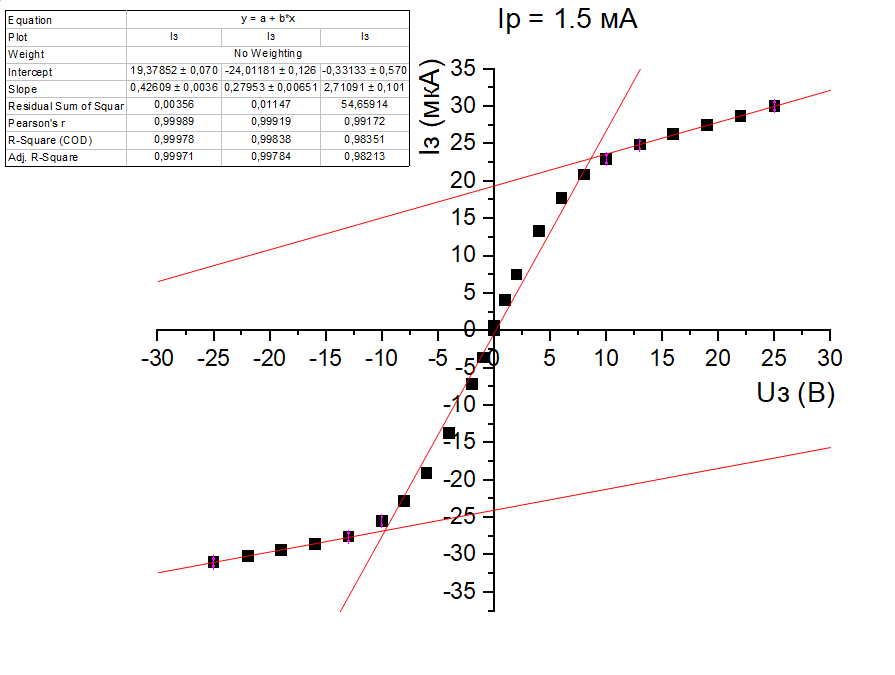
\includegraphics[width=0.95\textwidth]{3.5.1_11.png}\\
(c) ВАХ двойного зонда, $I_{p} = 1.5$ мА  \\
\end{center}

\begin{center}
\textbf{Рис. 9} Зондовые характеристики при различных токах разряда
\end{center}

\hfill \break \textbf{Температура электронов} рассчитывается по уже упомянутой выше формуле:

$$
T_{e} = \frac{\Delta U}{2k},
$$

\hfill \break причем энергии 1 эВ соответствует температура порядка $11800$ К. Эта формула в системе СИ. Далее, полагая концентрации электронов и ионов равными ($n_{i} = n_{e} = n$), определим эти \textbf{концентрации} из формулы Бома:

$$
I_{i\text{н}} = 0.4n_{e}eS\sqrt{\frac{2kT_{e}}{m_{i}}}, \text{ } \rightarrow n_{e} = \frac{I_{i\text{н}}}{0.4eS}\sqrt{\frac{m_{i}}{2kT_{e}}},
$$

\hfill \break где $S = \pi dl = 3.26$ $\text{мм}^2$ $-$ площадь поверхности зонда, $m_{i} = 22 \cdot 1.66 \cdot 10^{-27}$ кг $-$ масса иона неона. Эта формула также в СИ.

\hfill \break Также мы можем рассчитать \textbf{плазменную (ленгмюровскую) частоту} $\omega_{p}$ (в СГС) по формуле (1):

$$
\omega_{p} = \sqrt{\frac{4\pi n_{e}e^2}{m_{e}}} = 5.6 \cdot 10^4 \sqrt{n_{e}},
$$

\hfill \break где $m_{e} = 9.1 \cdot 10^{-28}$ г $-$ масса электрона, \textbf{электронную поляризационную длину} (в СГС):

$$
r_{De} = \sqrt{\frac{kT_{e}}{4\pi n_{e}e^2}} \text{ } \text{см},
$$

\hfill \break и \textbf{дебаевский радиус экранирования}:

$$
r_{D} = \sqrt{\frac{kT_{i}}{4\pi n_{e}e^2}} \text{ } \text{см},
$$

\hfill \break где считаем, что $T_{e} \gg T_{i}$, $T_{i} \approx 300$ К. Среднее \textbf{число ионов в дебаевской сфере} рассчитывается по формуле

$$
N_{D} = \frac{4}{3}\pi r_{D}^3n_{i},
$$

\hfill \break а \textbf{степень ионизации}, считая давление в трубке приблизительно равным 2 торр (2 мм рт. ст.), можно найти как $\alpha = n_{i}/n$, где $n$ $-$ общее число частиц в единице объема ($P = nkT_{i}$).

\hfill \break Теперь разберемся с погрешностями:

$$
\varepsilon_{n_{e}} \approx \sqrt{\frac{1}{4}\varepsilon_{T_{e}}^2+\varepsilon_{I_{i\text{н}}}^2};
$$
$$
\varepsilon_{T_{e}} \approx \varepsilon_{\Delta U};
$$
$$
\varepsilon_{\omega_{p}} \approx \frac{1}{2}\varepsilon_{n_{e}};
$$
$$
\varepsilon_{r_{De}} \approx \sqrt{\frac{1}{4}\varepsilon_{T_{e}}^2+\frac{1}{4}\varepsilon_{n_{e}}^2};
$$
$$
\varepsilon_{r_{D}} \approx \frac{1}{2} \varepsilon{n_{e}};
$$
$$
\varepsilon_{N_{D}} \approx \sqrt{\frac{1}{9}\varepsilon_{r_{D}}^2+\varepsilon_{n_{e}}^2};
$$
$$
\varepsilon_{\alpha} \approx \varepsilon_{n_{e}}.
$$

\hfill \break Наборы расчетов для трех различных токов разряда сведены в таблицу 3:

\begin{center}
\begin{tabular}{|c|c|c|c|c|c|c|c|}\hline
$I_p$, мА & $T_e \cdot 10^4$, К & $n_e\cdot10^{-9}$, $\text{cм}^{-3}$ & $\omega_p\cdot10^{-9}$, рад/с & $r_{D_e}$, мкм & $r_D$, мкм & $N_d$ & $\alpha \cdot 10^{-6}$ \\\hline
1.5  & 4.1 \pm 0.2 & 21.9 \pm 2.2 &  8.2 \pm 0.4 & 67.9 \pm 13.6 & 5.7 \pm 0.3 & 17.1 & 0.35 \\\hline
3.0  & 4.6 \pm 0.2 & 42.5 \pm 4.2 & 11.7 \pm 0.6 & 51.5 \pm 10.3 & 4.1 \pm 0.2 & 12.3 & 0.67 \\\hline
5.0  & 5.4 \pm 0.3 & 70.3 \pm 7.0 & 14.0 \pm 0.7 & 43.2 \pm 8.6 & 3.2 \pm 0.2 &  9.6 & 1.11 \\\hline
\end{tabular} \\
\hfill \break \textbf {Таблица 3.} Характеристики плазмы\\
\end{center}

\hfill \break По полученным результатам построим график зависимости электронной температуры от тока разряда $T_{e} (I_{p})$:

\begin{center}
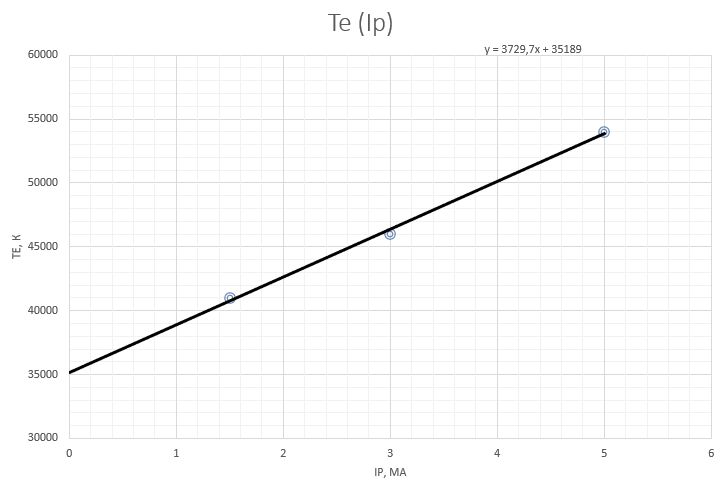
\includegraphics[width=0.95\textwidth]{3.5.1_12.png}\\
\textbf{Рис. 10.} График зависимости электронной температуры от тока разряда \\
\end{center}

\hfill \break Уравнение полученной зависимости указано на графике. Также построим график зависимости концентрации электронов от тока разряда:

\begin{center}
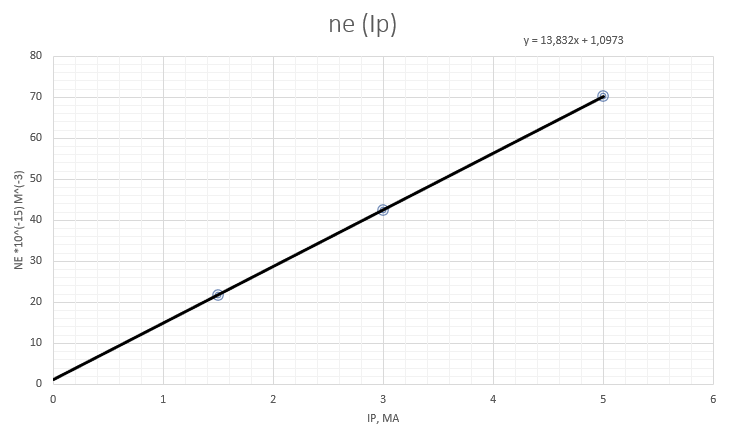
\includegraphics[width=0.95\textwidth]{3.5.1_13.png}\\
\textbf{Рис. 11.} График зависимости концентрации электронов от тока разряда \\
\end{center}

\hfill \break В заключение для наглядности построим на одном графике семейство зондовых характеристик для разных токов разряда:

\begin{center}
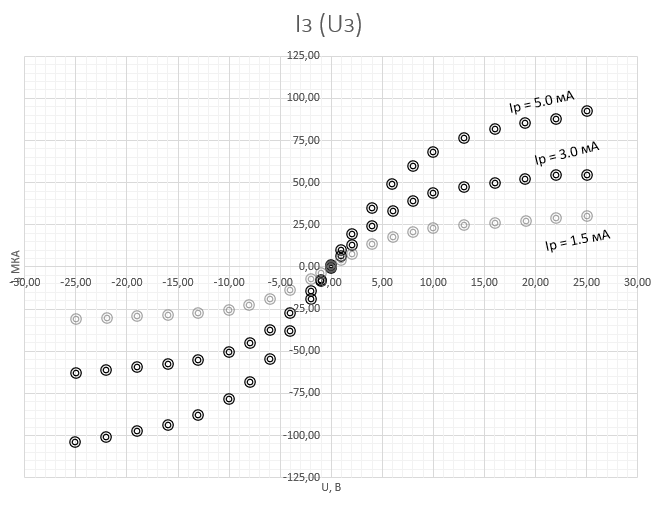
\includegraphics[width=0.95\textwidth]{3.5.1_14.png}\\
\textbf{Рис. 12.} Семейство зондовых характеристик \\
\end{center}

\section{Вывод}
\hfill \break В ходе работы была получена вольт-амперная характеристика тлеющего газового разряда, в результате чего было определено максимальное дифференциальное сопротивление разряда $R_\text{диф} = (6.15 \pm 0.24) \cdot 10^4$ Ом. Также были определены и рассчитаны характеристики плазмы при трех различных токах разряда (таблица 3). Из них можно сделать следующие выводы:
\begin{enumerate}
\item{степень ионизации достаточно далека от единицы, что соответствует температуре электронов порядка $10^4$ К;}
\item{так как $N_{D} \gg 1$, плазма близка к идеальной, потому что является очень разреженной;}
\item{так как дебаевский радиус очень мал (много меньше линейных размеров плазмы), плазму можно считать квазинейтральной.}
\end{enumerate}

\end{document}
